% Tamaño de letra.
\documentclass[12pt,titlepage]{report}

%------------------------------ Paquetes ----------------------------------

% Paquetes:

%Para comentarios multilínea.
\usepackage{verbatim}

% Para tener cabecera y pie de página con un estilo personalizado.
\usepackage{fancyhdr}

% Codificación UTF-8
\usepackage[utf8]{inputenc}

% Castellano.
\usepackage[spanish]{babel}

% Tamaño de página y márgenes.
\usepackage[a4paper,headheight=16pt,scale={0.75,0.8},hoffset=0.5cm]{geometry}

% Para poder agregar notas al pie en tablas:
%\usepackage{threeparttable}

% Tipo de letra Helvetica (Arial).
%\usepackage{helvet}
%\renewcommand\familydefault{\sfdefault}

% Gráficos:

% Para incluir imágenes, el siguiente código carga el paquete graphicx
% según se esté generando un archivo dvi o un pdf (con pdflatex).

% Para generar dv.
%\usepackage[dvips]{graphicx}

% Para generar pdf.
\usepackage[pdftex]{graphicx}
\pdfcompresslevel=9

\usepackage{pdfpages}

%
% Directorio donde están las imagenes.
%
%\newcommand{\imgdir}{includes}
%\graphicspath{{\imgdir/}}

%------------------------------ ~paquetes ---------------------------------

%------------------------- Inicio del documento ---------------------------

\begin{document}

% ---------------------- Encabezado y pie de página -----------------------

% Encabezado: sección a la derecha.
% Pie de página: número de página a la derecha.

\pagestyle{fancy}
\renewcommand{\sectionmark}[1]{\markboth{}{\thesection\ \ #1}}
\lhead{}
\chead{}
\rhead{\rightmark}
\lfoot{}
\cfoot{}
\rfoot{\thepage}

% ---------------------- ~Encabezado y pie de página ----------------------

% -------------------------- Título y autor(es) ---------------------------

\title{Información en las organizaciones}
\author{}

% -------------------------- ~Título y autor(es) --------------------------

% ------------------------------- Carátula --------------------------------

\begin{titlepage}

\thispagestyle{empty}

% Logo facultad más pie de la figura.
\begin{center}

\includegraphics[scale=0.55]{./Images/fiuba}\\
\large{\textsc{Universidad de Buenos Aires}}\\
\large{\textsc{Facultad De Ingeniería}}\\
\small{Año 2012 - 1\textsuperscript{er} Cuatrimestre}
\end{center}

\vfill

% Título central.
\begin{center}

\Large{\underline{\textsc{Información en las organizaciones (71.13)}}}

\vfill

% Tabla de integrantes.

\Large{\underline{\textsc{Trabajo Práctico}}}
\vfill

\Large\underline{Ayudante: Licenciada Paez} \linebreak\linebreak
\Large\underline{Integrantes Grupo 2} \linebreak\linebreak

% Separación entre columnas.
\large\addtolength{\tabcolsep}{-3pt}
% Tres columnas con alineación centrada.
\begin{tabular}{|| c | c | c ||}
\hline
\textbf{Apellido, Nombre} & \textbf{Nro. Padrón} & \textbf{E-mail} \\
\hline
Berrilio, Pablo & 88812 & pabloberrilio@gmail.com \\
\hline
Bukaczewski, Verónica & 86954 & vero13@gmail.com \\
\hline
De Antoni, Matías & 88506 & mdeantoni87@gmail.com \\
\hline
Garbarini, Lucía & 88300 & lu.teddy@gmail.com\\
\hline
Invernizzi, Esteban Ignacio & 88817 & invernizzie@gmail.com\\
\hline
Mouso, Nicolás Gastón & 88528 & nicolasgnr@gmail.com \\
\hline
Ygounet, Guido N. & 88246 & gygounet@gmail.com \\
\hline
Zelechowski, Sergio & 86651 & sergiozz123@gmail.com \\
\hline
Moreno Salas, Josué Fabio & Intercambio & josue.nalgarito@gmail.com \\
\hline
\end{tabular}
\end{center}

\vfill

\hrule
\vspace{0.2cm}

% Pie de página de la carátula.
\noindent\small{71.13 - Información en las organizaciones \hfill Grupo 2}

\end{titlepage}

% ------------------------------- ~Carátula -------------------------------

% -------------------------------- Índice ---------------------------------

% Hago que las páginas se comiencen a contar a partir de aquí.
\setcounter{page}{1}

% Índice.
\tableofcontents
\newpage

% -------------------------------- ~Índice --------------------------------

% ----------------------------- Inicio del tp -----------------------------

% Introducción.
%\chapter*{Introducción}
%\addcontentsline{toc}{chapter}{Introducción}

\part{Práctica}

\chapter{Práctica 1}

%\include{Practica/Practica1}

\part{Análisis de Empresa}
\chapter*{Enunciado}
Enunciado del trabajo práctico...

\chapter{Elección de la empresa}

% TABLA COMPARATIVA
\section{Tabla comparativa de empresas}
\begin{center}
\small\addtolength{\tabcolsep}{-5pt}
\begin{tabular}{|| c || c || c | c | c | c | c ||}
\hline
\hline
T\'{e}rminos & Peso & Empresa 1 & Empresa 2 & Empresa 3 & Empresa 4 & Empresa 5\\
\hline
Contacto   & 10 & 9 & 8 & 10 & 10 & 8 \\
\hline
Ubicaci\'{o}n & 7 & 6 & 10 & 5 & 6 & 7 \\
\hline
Tama\~{n}o & 8 & 9 & 8 & 8 & 3 & 8 \\
\hline
Disp. de info. & 10 & 9 & 6 & 10 & 8 & 8 \\
\hline
Centralizaci\'{o}n & 4 & 8 & 8 & 7 & 6 & 8 \\
\hline
\hline
Totales & - & 326 & 306 & 327 & 270 & 305 \\
\hline
\end{tabular}
\end{center}

%\pagebreak

% ELECCIÓN FINAL.

\section{Elección de la empresa}
Se eligió la empresa \textbf{Empresa X}, principalmente por haber obtenido el mejor puntaje según el criterio de comparación elegido. La buena calidad del contacto y la exelente disponibilidad de información situa a esta empresa por encima de otras propuestas.

\pagebreak


\chapter{Actividad de la empresa IEP De Iluminación}

\begin{center}
 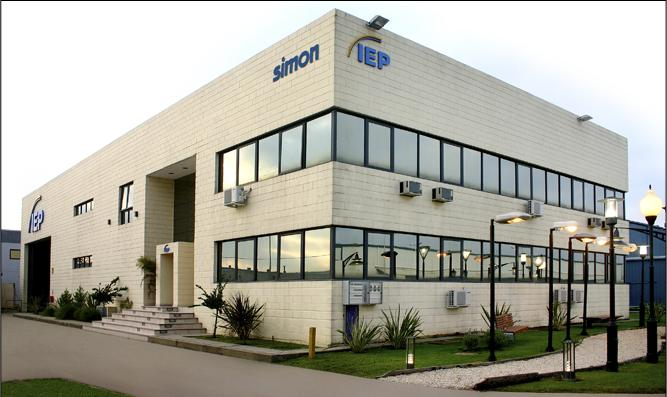
\includegraphics[scale=0.75]{./Images/iep-instalacion.png}
\end{center}

\section{Introducci\'on}
\subsection{Descripción}
Es una empresa multinacional dedicada a la fabricación y comercialización de luminarias, farolas, columnas y soportes, que ofrece soluciones de excelente calidad luminotécnica en Alumbrado Público, Áreas Verdes, Alumbrado Industrial, Alumbrado Interior, Alumbrado de Jardín, Iluminación con Sumergibles y Leds.

\subsection{Ubicación}
La empresa se encuentra ubicada en las afueras de la Ciudad de Buenos Aires, m\'as precisamente en el conurbano bonaerense en el kil\'ometro 37.5 del ramal Escobar de la Ruta Panamericana. A pesar de encontrarse a aproximadamente 
40 kil\'ometros de la Capital Federal, es relativamente f\'acil y r\'apido llegar hasta la f\'abrica.

\subsection{Historia}
En el año 1922 Industrias Electrotécnicas Puig (IEP) se especializaba en la fabricación de aparatos reflectores para alumbrado en la española ciudad de Barcelona.
En el año 1966 pasa a formar parte del Grupo Simon, un holding de empresas del mercado eléctrico español con visionaria expansión hacia a los cinco continentes.
A principios de la década del 90 adapta nuevamente su estructura y su imagen, empezando a conocérsela como IEP DE ILUMINACIÓN.
Es en el año 1998 que IEP DE ILUMINACIÓN llega a la Argentina, convirtiéndose en el lapso de 12 años en la principal responsable de la comercialización de luminarias para toda América del Sur. 
Como en todo proceso de expansión y desarrollo, el Grupo Simon fue incorporando nuevos centros de producción y filiales en Latinoamérica (Argentina, Brasil y México), en Europa (Francia, Reino Unido, Irlanda, Bélgica, Holanda, Noruega, Suiza, Polonia), en África (Marruecos y Egipto) y en Asia (China, India, Rusia, Turquía) para poder llegar con mayor rapidez y eficiencia operativa a todos sus mercados.
En la actualidad cuenta con 24 empresas coordinadas desde su sede central en Barcelona (España) y su presencia mundial alcanza a más de 50 países. Centra sus actividades en el ámbito de la instalación eléctrica con diversas líneas de productos: material eléctrico y protección de circuitos, iluminación, domótica, conexiones para voz y datos, canalizaciones y electrónica. Las más recientes incorporaciones en su línea de negocios comprenden el mobiliario urbano y la seguridad. El primero por su relación con los espacios de iluminación urbana y el segundo porque las innovaciones aplicadas en este campo también incluyen material eléctrico.

\subsubsection{En Argentina}
Durante sus primeros años de actividad en el país, la empresa contó con planta de producción en la localidad de Munro (Buenos Aires) y oficinas comerciales en San Isidro (Buenos Aires), pero el creciente aumento de los volúmenes de venta fundados en la producción de luminarias de avanzada tecnología y diseños de vanguardia, demandó la instalación de una planta fabril de mayor tamaño y capacidad productiva.
Así, posicionada en el ámbito local como la empresa “Líder en Innovación Tecnológica”, IEP DE ILUMINACIÓN cuenta desde el año 2005 con instalaciones propias dentro del Centro Industrial Garín (Buenos Aires), garantizando rapidez operativa y de organización al reunir en un mismo lugar tanto sus áreas Comerciales como las de Producción y Almacenamiento.

\section{Filosof\'ia de la empresa}

\subsection{Misi\'on}

La misi\'on de la empresa consiste en operar un sistema rentable que les permita satisfacer las necesidades actuales y potenciales del mercado luminot\'ecnico, 
ofreciendo productos y servicios con verdadero valor agregado, a fin de construir relaciones fuertes y a largo plazo.

\subsection{Visi\'on}

La empresa define su visi\'on de la siguiente forma:\\
Ser considerada la empresa de iluminaci\'on m\'as pujante convirtiendonos en el proveedor preferido por el mercado luminot\'ecnico al ofrecer los mejores 
productos y servicios del rubro.
 
\section{Estructura de la empresa}

\subsection{Organigrama}
A continuación se presenta el organigrama completo de la empresa. Ver imagen \ref{organigramaIEP}

\begin{figure}[h!]
  \centering
  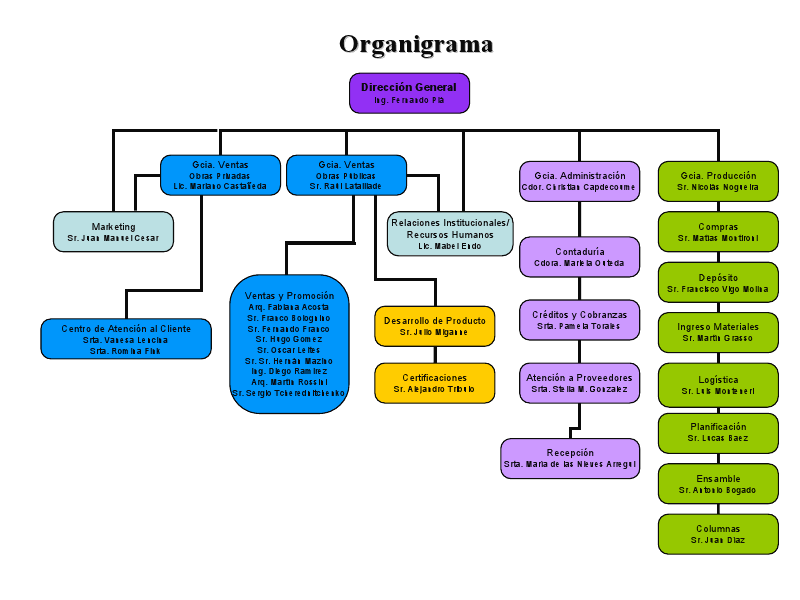
\includegraphics[scale=0.55]{./Images/organigrama.png}
  \caption{Organigrama IEP}\label{organigramaIEP}
\end{figure}

% Para incluir un pdf usar:
%\includepdf[pages=1-19, scale=0.7]{*.pdf}

% ------------------------------ Fin del tp -------------------------------

\end{document}

%---------------------------- Fin del documento ---------------------------
